\documentclass{article}\usepackage[]{graphicx}\usepackage[]{color}
%% maxwidth is the original width if it is less than linewidth
%% otherwise use linewidth (to make sure the graphics do not exceed the margin)
\makeatletter
\def\maxwidth{ %
  \ifdim\Gin@nat@width>\linewidth
    \linewidth
  \else
    \Gin@nat@width
  \fi
}
\makeatother

\definecolor{fgcolor}{rgb}{0.345, 0.345, 0.345}
\newcommand{\hlnum}[1]{\textcolor[rgb]{0.686,0.059,0.569}{#1}}%
\newcommand{\hlstr}[1]{\textcolor[rgb]{0.192,0.494,0.8}{#1}}%
\newcommand{\hlcom}[1]{\textcolor[rgb]{0.678,0.584,0.686}{\textit{#1}}}%
\newcommand{\hlopt}[1]{\textcolor[rgb]{0,0,0}{#1}}%
\newcommand{\hlstd}[1]{\textcolor[rgb]{0.345,0.345,0.345}{#1}}%
\newcommand{\hlkwa}[1]{\textcolor[rgb]{0.161,0.373,0.58}{\textbf{#1}}}%
\newcommand{\hlkwb}[1]{\textcolor[rgb]{0.69,0.353,0.396}{#1}}%
\newcommand{\hlkwc}[1]{\textcolor[rgb]{0.333,0.667,0.333}{#1}}%
\newcommand{\hlkwd}[1]{\textcolor[rgb]{0.737,0.353,0.396}{\textbf{#1}}}%

\usepackage{framed}
\makeatletter
\newenvironment{kframe}{%
 \def\at@end@of@kframe{}%
 \ifinner\ifhmode%
  \def\at@end@of@kframe{\end{minipage}}%
  \begin{minipage}{\columnwidth}%
 \fi\fi%
 \def\FrameCommand##1{\hskip\@totalleftmargin \hskip-\fboxsep
 \colorbox{shadecolor}{##1}\hskip-\fboxsep
     % There is no \\@totalrightmargin, so:
     \hskip-\linewidth \hskip-\@totalleftmargin \hskip\columnwidth}%
 \MakeFramed {\advance\hsize-\width
   \@totalleftmargin\z@ \linewidth\hsize
   \@setminipage}}%
 {\par\unskip\endMakeFramed%
 \at@end@of@kframe}
\makeatother

\definecolor{shadecolor}{rgb}{.97, .97, .97}
\definecolor{messagecolor}{rgb}{0, 0, 0}
\definecolor{warningcolor}{rgb}{1, 0, 1}
\definecolor{errorcolor}{rgb}{1, 0, 0}
\newenvironment{knitrout}{}{} % an empty environment to be redefined in TeX

\usepackage{alltt}
\usepackage[margin=0.5in]{geometry}
\usepackage{boxedminipage}
\usepackage{amsfonts}
\usepackage{amsmath} 
\usepackage{amssymb}
\usepackage{graphicx}
\usepackage{amsthm}
\usepackage{t1enc}
\usepackage{subfig}
\IfFileExists{upquote.sty}{\usepackage{upquote}}{}
\begin{document}
\title{\color{red}HW1 - STAT 580 - Sp 2015}
\author{Yet T Nguyen}
\date{01/29/2015}
\maketitle

\section*{1.}
\begin{verbatim}
#include <stdio.h>
#include <math.h>
#define P0 0.01 /* lower limit of the probability (p)*/
#define P1 0.5 /* upper limit of the probability (p)*/
#define PLEN 10 /* number of columns*/
#define N 5 /* number of experiments (n)*/


int fact(int n); /*funtion to calculate factorial of n*/

int main(){
  int x = 0; 
  float dist, p;
  p = P0;
  dist = (P1-P0)/(PLEN-1);
  printf("x\\p\t"); 
  for (p = P0; p <= P1; p+= dist){
    printf("%.4f ", p); /* print p values*/
  }
  printf("\n\v"); /* print vertical tab */
  for (x = 0; x <= N; x++){
    printf("%d  \t", x);
    for (p = P0; p <= P1; p+= dist){
      printf("%.4f ", fact(N)/(fact(x)*fact(N-x))*pow(p,x)*pow(1-p, N-x)); /*print probabilites*/
    }
    printf("\n");
  }
  return 0;
}

int fact(int n){
  int out = 1;
  if (n ==0) out = 1;
  while (n >= 1){
    out = out*n;
    n--;
  }
  return out;
}
\end{verbatim}
% \begin{verbatim}
% 
% x\p  0.0100 0.0644 0.1189 0.1733 0.2278 0.2822 0.3367 0.3911 0.4456 0.5000 
% 
% 0  	 0.9510 0.7167 0.5311 0.3861 0.2746 0.1905 0.1284 0.0837 0.0524 0.0313 
% 1  	 0.0480 0.2469 0.3583 0.4047 0.4050 0.3746 0.3259 0.2688 0.2105 0.1563 
% 2  	 0.0010 0.0340 0.0967 0.1697 0.2389 0.2945 0.3308 0.3453 0.3384 0.3125 
% 3  	 0.0000 0.0023 0.0130 0.0356 0.0705 0.1158 0.1679 0.2218 0.2719 0.3125 
% 4  	 0.0000 0.0001 0.0009 0.0037 0.0104 0.0228 0.0426 0.0712 0.1093 0.1562 
% 5  	 0.0000 0.0000 0.0000 0.0002 0.0006 0.0018 0.0043 0.0092 0.0176 0.0312 
% \end{verbatim}
\section*{2.}
\begin{itemize}
\item[(a)] We have 
\begin{align*}
&f(x) \propto \exp(-x) \quad 0<x<2\\
& \Rightarrow F(x) = (1-\exp(-x))/(1-exp(-2)) \quad 0<x<2\\
& \Rightarrow F^{-1}(u) = -\log(1-(1-\exp(-2))u) \quad 0<u<1.
\end{align*}
The simulation algorithm is as below
\begin{itemize}
\item Generate a uniform random variable $u$.
\item The variable $X \equiv F^{-1}(u)$ will has the requried distribution.
\end{itemize}
\item[(b)]
\begin{verbatim}
#include <stdio.h>
#include <time.h>
#define MATHLIB_STANDALONE
#include <Rmath.h>
int main() {
  double u, x;
  set_seed(time(NULL), 580580); /* set seed */
    u = unif_rand(); /* uniform random variable */
    x = -log(1- (1-exp(-2))*u);
    printf("%f\n ", x);
    return 0;
    }
\end{verbatim}
\item[(c)]
\begin{knitrout}
\definecolor{shadecolor}{rgb}{0.969, 0.969, 0.969}\color{fgcolor}\begin{kframe}
\begin{alltt}
\hlstd{u} \hlkwb{<-} \hlkwd{runif}\hlstd{(}\hlnum{5000}\hlstd{,} \hlnum{0}\hlstd{,} \hlnum{1}\hlstd{)}

\hlstd{x} \hlkwb{<-} \hlopt{-}\hlkwd{log}\hlstd{(}\hlnum{1}\hlopt{-}\hlstd{(}\hlnum{1}\hlopt{-}\hlkwd{exp}\hlstd{(}\hlopt{-}\hlnum{2}\hlstd{))}\hlopt{*}\hlstd{u)}
\hlkwd{hist}\hlstd{(x,} \hlkwc{prob} \hlstd{= T,} \hlkwc{nclass} \hlstd{=} \hlnum{100}\hlstd{)}
\hlkwd{lines}\hlstd{(}\hlkwd{density}\hlstd{(x),} \hlkwc{col} \hlstd{=} \hlstr{"red"}\hlstd{)}
\end{alltt}
\end{kframe}

{\centering 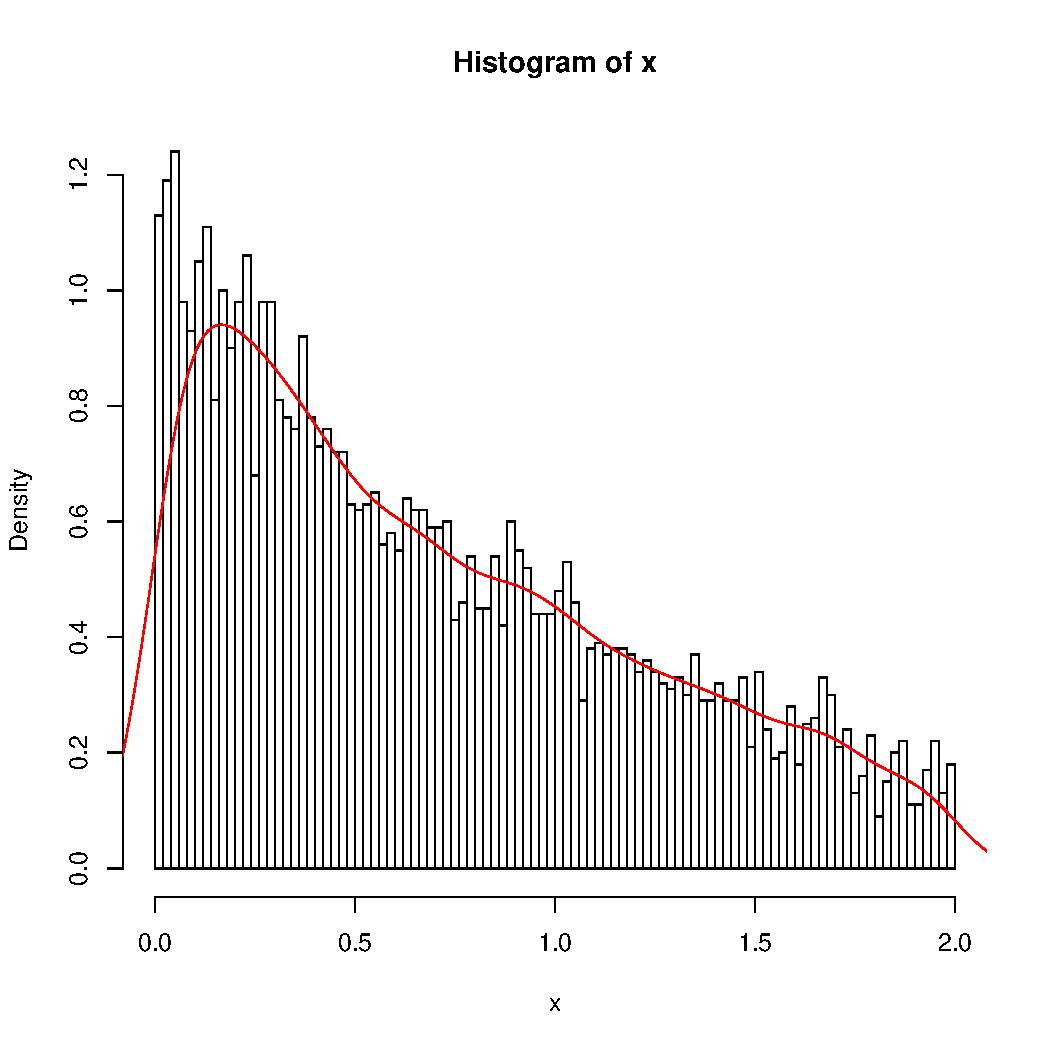
\includegraphics[width=\maxwidth]{figure/unnamed-chunk-1-1} 

}



\end{knitrout}
\end{itemize}

\section*{3.}
\begin{itemize}
\item[(a)]
\begin{knitrout}
\definecolor{shadecolor}{rgb}{0.969, 0.969, 0.969}\color{fgcolor}\begin{kframe}
\begin{alltt}
\hlkwd{set.seed}\hlstd{(}\hlnum{1}\hlstd{)}
\hlstd{rs} \hlkwb{<-} \hlkwa{function}\hlstd{(}\hlkwc{g}\hlstd{)\{}
  \hlkwa{if} \hlstd{(g}\hlopt{==}\hlstr{"g1"}\hlstd{)\{}
    \hlkwa{repeat}\hlstd{\{}
      \hlstd{x} \hlkwb{<-} \hlkwd{rexp}\hlstd{(}\hlnum{1}\hlstd{,}\hlnum{1}\hlstd{)}
      \hlstd{u} \hlkwb{<-} \hlkwd{runif}\hlstd{(}\hlnum{1}\hlstd{,}\hlnum{0}\hlstd{,}\hlnum{1}\hlstd{)}
      \hlstd{r} \hlkwb{<-} \hlnum{1}\hlopt{/}\hlstd{(}\hlnum{1}\hlopt{+}\hlstd{x}\hlopt{^}\hlnum{2}\hlstd{)}
      \hlkwa{if} \hlstd{(u} \hlopt{<=} \hlstd{r)\{}
        \hlstd{res} \hlkwb{<-} \hlstd{x}
        \hlkwa{break}
      \hlstd{\}}
  \hlstd{\}}
  \hlstd{\}}
  \hlkwa{if} \hlstd{(g}\hlopt{==}\hlstr{"g2"}\hlstd{)\{}
    \hlkwa{repeat}\hlstd{\{}
      \hlstd{x} \hlkwb{<-} \hlkwd{abs}\hlstd{(}\hlkwd{rcauchy}\hlstd{(}\hlnum{1}\hlstd{,}\hlnum{0}\hlstd{,}\hlnum{1}\hlstd{))}
      \hlstd{u} \hlkwb{<-} \hlkwd{runif}\hlstd{(}\hlnum{1}\hlstd{,}\hlnum{0}\hlstd{,}\hlnum{1}\hlstd{)}
      \hlstd{r} \hlkwb{<-} \hlkwd{exp}\hlstd{(}\hlopt{-}\hlstd{x)}
      \hlkwa{if} \hlstd{(u} \hlopt{<=} \hlstd{r)\{}
        \hlstd{res} \hlkwb{<-} \hlstd{x}
        \hlkwa{break}
      \hlstd{\}}
    \hlstd{\}}
  \hlstd{\}}
  \hlstd{res}
\hlstd{\}}

\hlkwd{library}\hlstd{(plyr)}
\hlstd{n} \hlkwb{<-} \hlnum{5000}
\hlstd{pm1} \hlkwb{<-} \hlkwd{proc.time}\hlstd{()}
\hlstd{rs.g1} \hlkwb{<-} \hlkwd{laply}\hlstd{(}\hlnum{1}\hlopt{:}\hlstd{n,} \hlkwa{function}\hlstd{(}\hlkwc{i}\hlstd{)}\hlkwd{rs}\hlstd{(}\hlstr{"g1"}\hlstd{))}
\hlkwd{proc.time}\hlstd{()}\hlopt{-}\hlstd{pm1}
\end{alltt}
\begin{verbatim}
##    user  system elapsed 
##   0.119   0.000   0.124
\end{verbatim}
\begin{alltt}
\hlkwd{hist}\hlstd{(rs.g1,} \hlkwc{nclass} \hlstd{=} \hlnum{100}\hlstd{,} \hlkwc{prob} \hlstd{= T)}
\hlkwd{lines}\hlstd{(}\hlkwd{density}\hlstd{(rs.g1),} \hlkwc{col} \hlstd{=} \hlstr{"red"}\hlstd{)}
\hlstd{pm2} \hlkwb{<-} \hlkwd{proc.time}\hlstd{()}
\hlstd{rs.g2} \hlkwb{<-} \hlkwd{laply}\hlstd{(}\hlnum{1}\hlopt{:}\hlstd{n,} \hlkwa{function}\hlstd{(}\hlkwc{i}\hlstd{)}\hlkwd{rs}\hlstd{(}\hlstr{"g2"}\hlstd{))}
\hlkwd{proc.time}\hlstd{()}\hlopt{-}\hlstd{pm2}
\end{alltt}
\begin{verbatim}
##    user  system elapsed 
##   0.204   0.004   0.209
\end{verbatim}
\begin{alltt}
\hlkwd{hist}\hlstd{(rs.g2,} \hlkwc{nclass} \hlstd{=} \hlnum{100}\hlstd{,} \hlkwc{prob} \hlstd{= T)}
\hlkwd{lines}\hlstd{(}\hlkwd{density}\hlstd{(rs.g2),} \hlkwc{col} \hlstd{=} \hlstr{"red"}\hlstd{)}
\end{alltt}
\end{kframe}

{\centering 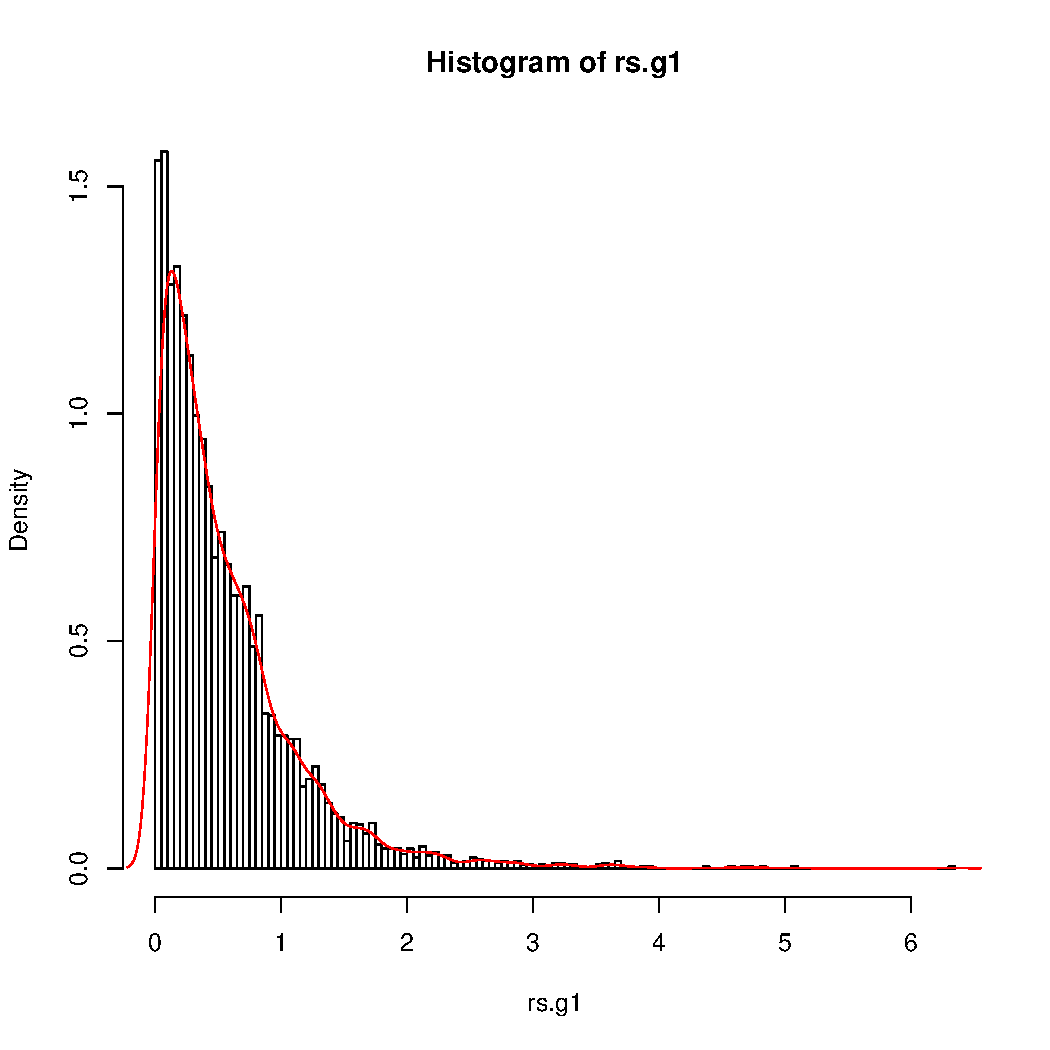
\includegraphics[width=8cm,height=8cm]{figure/unnamed-chunk-2-1} 
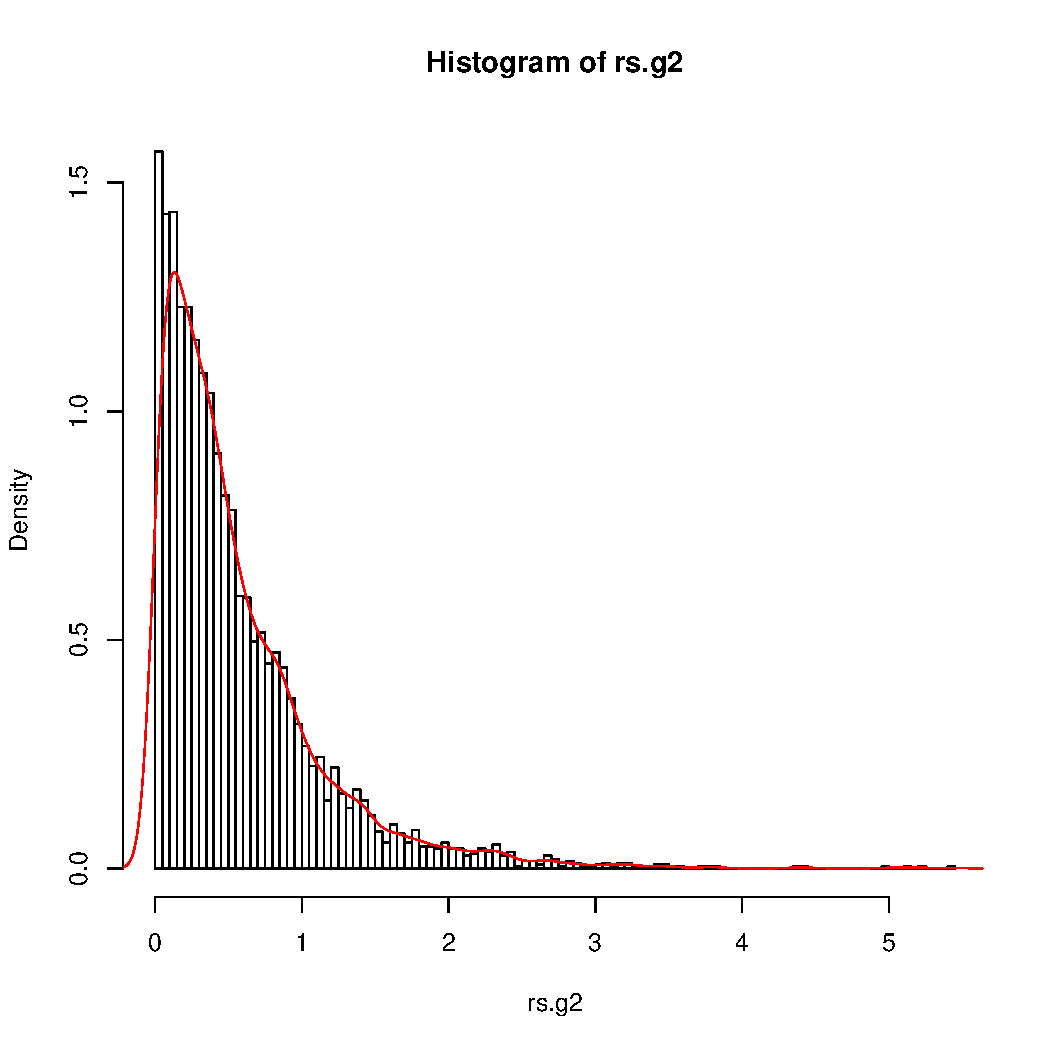
\includegraphics[width=8cm,height=8cm]{figure/unnamed-chunk-2-2} 

}



\end{knitrout}
\item[(b)] From the output, the algorithm using envelop density $g_1$ is faster than the one using envelop density $g_2$. The sampling results of those densities are similar.
\end{itemize}
\section*{4.}
We have 
\begin{align}
& f(x,y) \propto x^\alpha y \notag\\
&\Rightarrow f(x) \propto \int_{0<y<\sqrt{1-x^2}} x^\alpha y dy \propto x^\alpha(1-x^2)
\quad \mbox{ for } 0<x<1 \label{eq1}\\
&\mbox{and } f(y|x) \propto \frac{x^\alpha y}{x^\alpha(1-x^2)} \propto y \quad \mbox {for } y \leq \sqrt{1-x^2} \label{eq2}.
\end{align}

\eqref{eq1} implies that
\begin{equation}\label{eq3}
x^\alpha (1-x^2) \leq x^\alpha
\end{equation}
and \eqref{eq2} implies that
\begin{equation}\label{eq4}
F(y|x) = \frac{y^2}{1-x^2} \quad  0<y\leq 1-x^2, x>0
\end{equation}

From \eqref{eq3} and \eqref{eq4}, a rejection sampling algorithm to sample $(x,y)$ has distribution $f$ is as below

\begin{itemize}
\item First simulate $x$ with density $f_x \propto x^\alpha (1-x^2)$ by 

\begin{itemize}
 \item Simulate $z$ having the density $\propto z^\alpha$ $(0<z<1)$ by using the inverse transform method.
\item Using $z$ above as a proposal to simulate $x$ according to rejection sampling method.
\end{itemize}
\item Next, simulate $y|x$ having CDF as in \eqref{eq4} by using inverse transform method.
\end{itemize}

\end{document}
